\documentclass[12pt]{article}

% Custom Commands
\newcommand{\abs}[1]{\left| {#1} \right|}
\newcommand{\ceil}[1]{\lceil {#1} \rceil}
\newcommand{\floor}[1]{\lfloor {#1} \rfloor}
\newcommand{\paren}[1]{\left( {#1} \right)}
\newcommand{\series}[2]{\sum_{ {#1} }^{ {#2} }}

% Math and symbol packages
\usepackage{amsmath}
\usepackage{amsthm}
\usepackage{amssymb}
\usepackage{mathtools}
\usepackage{derivative}
\usepackage{tikz}
\usepackage{xcolor}
\usetikzlibrary{calc}

% Formatting
\usepackage{inputenc}
\usepackage[left=2.54cm,right=2.54cm,top=2.54cm,bottom=2.54cm]{geometry}
\usepackage{fancyhdr}
\usepackage{lipsum}
\usepackage{dashrule}

% Spacing formats
\AtBeginDocument{
	\setlength{\abovedisplayskip}{-2pt}
	\setlength{\belowdisplayskip}{5pt}
}

% Actual content
\begin{document}
\pagestyle{fancy}
\setlength{\headheight}{14.49998pt}
\fancyhead[L]{Trevor Swan}
\fancyhead[C]{\textbf{CSDS233 - HW2}}
\fancyhead[R]{10/08/24}
\fancyfoot[C]{\thepage}

% Begin Problem 1
\noindent \textbf{P.1) Answer the following questions:}

\noindent (a) Each element in an array occupies 4 storage units. If the storage address of the $20^{th}$ element is 500, what is the starting address of the array? (Give the calculation process or explanation.) \\

\indent Arrays have constant indexing as the different elements in the array have addresses varying by a constant value, which is 4 in this case. If the 20th element has an address of 500, then

$$
\begin{array}{|c|c|c|c|c|c|}
\hline
a_{n} & a_{n+4} & a_{n+8} & \dots & a_{496} & a_{500} \\
\hline
\end{array}
$$

\noindent is the array where $n$ is the first memory address and $a_{500}$ is the memory address of the 20th element. The address of an element in an array can be found by

$$ 
\text{(Element Address)}=\text{(Starting Address)}+(\text{Element Index})\cdot\text{(Storage per Element)}.
$$

It is important to note that an Element's Index is its number in the array minus 1 as java is a 0-based index language. We can find the starting address by $500 = 19(4) + n$, and can solve to get $n = 424$. Therefore the starting address of the array is $\boxed{424}$.

\noindent \hdashrule[0.5ex]{\textwidth}{1pt}{3mm 2mm}

\noindent (b) What do stacks and queues have in common? \\

\indent Stacks and Queues are both linear data structures like arrays and linked lists and both store collections of elements. They are both dynamic in size, so they can dynamically grow or shrink in size as elements are added and removed over time. They can both be implemented using other data structures, and specify the order in which elements are processed. For example, stacks follow "Last In, First Out" (LIFO), while queues follow "First In, First Out" (FIFO). These behaviors cause them to be useful for many algorithms.

\noindent \hdashrule[0.5ex]{\textwidth}{1pt}{3mm 2mm}

\noindent (c) For a binary tree with a depth of 8, what are the maximum and minimum possible numbers of nodes it can have? (Give the calculation process or explanation.) \\

\indent A minimal binary tree has only one node per level as each node only has one child. Therefore assuming the parent node is at depth 0, then there can be a minimum 9 nodes in a binary tree with depth $\boxed{8}$.

\indent A full binary tree, on the other hand, has 2 children per node. The number of nodes on any given level of a binary tree is given by $2^h$, where $h$ is the current level on the tree (0-based index). Therefore the total number of nodes is given by $2^0 + 2^1+2^2+\dots+2^8=\series{n=0}{8}2^n=\boxed{511}$.

\newpage

\noindent (d) A complete binary tree contains 256 nodes. What is its depth, and how many leaf nodes does it have? (Give the calculation process or explanation.) \\

\indent Generally, the total number of nodes in a tree can be found without using a summation as $N_{max}=2^{d+1}-1$, where $d$ is the depth of the tree. This is derived from the geometric series relation $S=\frac{a_1r^n-1}{r-1}$ where n is the total number of terms (the depth plus 1).

\indent We can solve for the depth of the tree by taking the floor function of d after solving for it as $d=\ceil{\frac{\ln\paren{N+1}}{\ln2}-1}$. Given that $N=256$, we find that $\boxed{d=8}$. We can solve for the total number of leaf nodes by observing that in a full binary tree with a depth of 7, there are $2^7=128$ leaf nodes. Also, a tree with a depth of 7 has 255 total nodes, and ours has 256. Therefore one of the nodes on the 7th level has a child, but there are still a total of $\boxed{128}$ leaf nodes on the tree.

\noindent \hdashrule[0.5ex]{\textwidth}{1pt}{3mm 2mm}

\noindent (e) If the input sequence of a stack is 1, 2, 3, 4, 5, 6, provide three possible output sequences.

\begin{enumerate}
	\item Push all $\to$ pop all.
	\begin{align*}
		6, 5, 4,& 3, 2, 1 && \text{Push all elements} \\
		\textbf{Output Sequence: } 6, 5, 4,& 3, 2, 1 && \text{Pop all elements}
	\end{align*}
	\item Pop midway through pushing elements. 
	\begin{align*}
		3, 2&, 1 && \text{Push 1, 2, 3 onto the stack} \\
		2,& 1 && \text{Pop 3} \\
		6, 5, 4&, 2, 1 && \text{Push the rest of the elements} \\
		\textbf{Output Sequence: } 3, 6, 5, 4&, 2, 1 && \text{Pop the rest of the stack}
	\end{align*}
	\item Alternate pushing and popping.
	\begin{align*}
		2,& 1 && \text{Push 1, 2 onto stack} \\
		1& && \text{Pop 2} \\
		4, 3&, 1 && \text{Push 3, 4 onto stack} \\
		3,& 1 && \text{Pop 4} \\
		6, 5,& 3, 1 && \text{Push 5, 6 onto stack} \\
		\textbf{Output Sequence: } 2, 4, 6, 5&, 3, 1 && \text{Pop the rest of the stack}
	\end{align*}
\end{enumerate}
\newpage

% Begin Problem 2
\noindent \textbf{P.2) Consider the following binary tree with 15 nodes. Describe the order of nodes visited in each of
the following traversals of the tree:}

\begin{center}
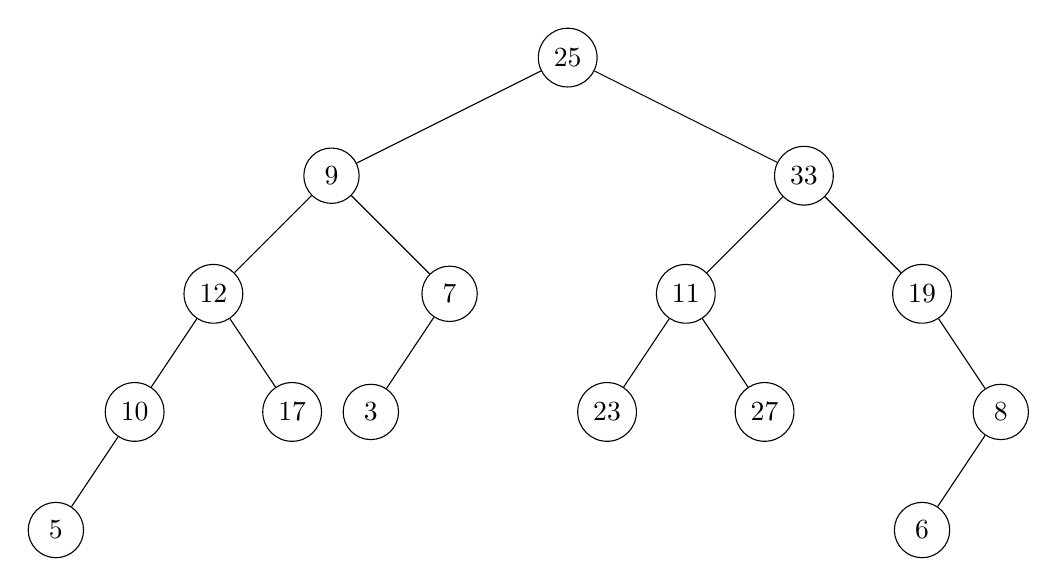
\begin{tikzpicture}[
	every node/.style = {minimum width = 2em, draw, circle},
	level 1/.style = {sibling distance = 60mm},
	level 2/.style = {sibling distance = 30mm},
	level 3/.style = {sibling distance = 20mm}
]
\node{25}
child {node {9}
	child {node {12}
		child {node {10}
			child {node {5}}
			child [missing]
		}
		child {node {17}}
	}
	child {node {7}
		child {node {3}}
		child [missing]
	}
}
child {node {33}
	child {node {11}
		child {node {23}}
		child {node {27}}	
	}
	child {node {19}
		child [missing]
		child {node {8}
			child {node {6}}
			child [missing]
		}
	}
};
\end{tikzpicture}
\end{center}

\noindent (a) In-Order

\noindent Nodes are visited in Left-Root-Right order. This gives:

\begin{align*}
	\boxed{5, 10, 12, 17, 9, 3, 7, 25, 23, 11, 27, 33, 19, 6, 8}
\end{align*} 

\noindent \hdashrule[0.5ex]{\textwidth}{1pt}{3mm 2mm}

\noindent (b) Pre-Order

\noindent Nodes are visited in Root-Left-Right order. This gives:

\begin{align*}
	\boxed{25, 9, 12, 10, 5, 17, 7, 3, 33, 11, 23, 27, 19, 8, 6}
\end{align*} 

\noindent \hdashrule[0.5ex]{\textwidth}{1pt}{3mm 2mm}

\noindent (c) Post-Order

\noindent Nodes are visited in Left-Right-Root order. This gives:

\begin{align*}
	\boxed{5, 10, 17, 12, 3, 7, 9, 23, 27, 11, 6, 8, 19, 33, 25}
\end{align*} 

\newpage

% Begin Problem 3
\noindent \textbf{P.3) Convert the following expressions from infix into postfix or from postfix into infix.} \textit{(Use PEMDAS to convert expressions)} \\

\noindent (a) 7 / 5 * G \^{} 6 * C + A \^{} 3 * B + Z - T

\noindent This expression is in infix, and should be converted to postfix as follows:

\begin{align*}
	\boxed{\text{7 5 / G 6 \^{} * C * A 3 \^{} B * + Z + T -}}
\end{align*}

\noindent \hdashrule[0.5ex]{\textwidth}{1pt}{3mm 2mm}

\noindent (b) X * Y$^2$ * $\frac{7}{\sqrt{1-\frac{\text{A}^2}{\text{B}^2}}}$ - Z

\noindent We can first rewrite this so that its easier to work with as: 

\begin{align*}
	\text{X * Y \^{} 2 * 7 / (1 - A \^{} 2 / B \^{} 2) \^{} 0.5 - Z}
\end{align*}

\noindent This expression is in infix, and should be converted to postfix as follows:

\begin{align*}
	\boxed{\text{X Y 2 \^{} * 7 * 1 A 2 \^{} B 2 \^{} / - 0.5 \^{} / Z -}}
\end{align*}

\noindent \hdashrule[0.5ex]{\textwidth}{1pt}{3mm 2mm}

\noindent (c) X Y Z - / A 8 O P Q / - * G 2 \^{} * / -

\noindent This expression is in postfix, and should be converted to infix as follows:

\begin{align*}
	\boxed{\text{X / (Y - Z) - A / (8 * (O - P / Q) * G \^{} 2)}}
\end{align*}

\noindent \hdashrule[0.5ex]{\textwidth}{1pt}{3mm 2mm}

\noindent (d) b 2 - 4 a c * - 2 a * / + 7 c * +

\noindent This expression is in postfix, and should be converted to infix as follows:

\begin{align*}
	\boxed{\text{b - 2 + (4 - a * c) / (2 * a) + 7 * c}}
\end{align*}

\end{document}
